\newpage
\section{Wyniki symulacji} \label{initial_phase_section}
\subsection{Wyznaczenie długości fazy początkowej}
Długość fazy początkowej wyznaczono za pomocą binarnego pliku \emph{log} zawierającego ilość zajętych bloków zasobów każdej stacji w funkcji czasu. Uzyskane wyniki dla pięciu różnych wartości parametru $\lambda$ przedstawiono w tabeli \ref{initial_phase_table}. Na podstawie uzyskanych wyników stwierdzono skracanie czasu trwania fazy początkowej wraz ze wzrostem wartości parametru $\lambda$ oraz uznano jej wpływ na wyniki trwania eksperymentu za nieznaczące. Przykładowy wykres, na podstawie którego wyznaczono wyniki przedstawiono na rysunku \ref{initial_phase_lambda_20}. Analizując wyniki należy mieć na uwadze subiektywność uzyskanych wyników, ze względu na nieprecyzyjną definicję końca fazy początkowej.

\begin{table}[h]
\caption{Wyznaczony czas fazy początkowe dla różnych wartości $\lambda$}
\label{initial_phase_table}
\begin{center}
\renewcommand{\arraystretch}{1.5}
\begin{tabular}{|l|l|l|l|l|l|}
\hline 
Lambda & 20 & 25 & 30 & 35 & 40 \\ 
\hline 
Czas fazy początkowej [s] & 38 & 36 & 30 & 27 & 20 \\ 
\hline
\end{tabular}
\end{center}
\end{table}

\begin{figure}[h]
\center
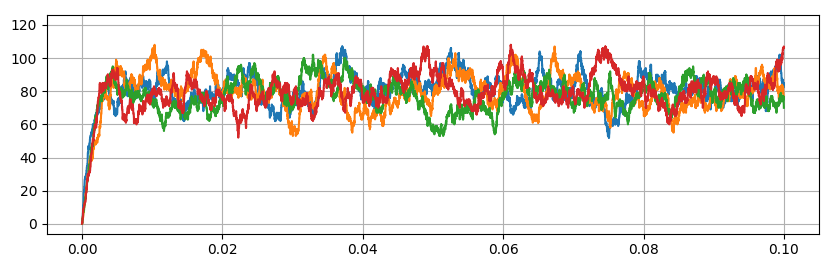
\includegraphics[scale=0.65]{img/initial_phase_lambda_20.png} 
\caption{Wykres ilości zajętych bloków zasobów stacji bazowych w funkcji czasu wyrażonego w godzinach. Parametr $\lambda$ podczas symulacji był równy 20}
\label{initial_phase_lambda_20}
\end{figure}

\subsection{Wyznaczenie granicznej wartości $\lambda$, dla której nie stracono żadnego użytkownika}
Aby wyznaczyć wartość graniczną, uruchomiono symulację dla wartości $\lambda$ z zakresu $<10; 50>$ użytkowników na sekundę, z krokiem 5. Każda próbka została uśredniona z 10 iteracji. W trakcie symulacji logika odpowiadająca za usypianie stacji była wyłączona. Wyniki symulacji, wraz z obliczonymi przedziałami ufności, przedstawiono w tabeli \ref{dropped_users_by_lambda_table} oraz na rysunku \ref{dropped_users_lambda}. Ostatnią wyznaczoną wartością $\lambda$, dla której nie stracono żadnego użytkownika, to 30 użytkowników na sekundę.

\begin{table}[]
\centering
\renewcommand{\arraystretch}{1.5}
\caption{Wyniki pomiaru ilości traconych użytkowników w systemie w funkcji wartości parametru $\lambda$}
\label{dropped_users_by_lambda_table}
\begin{tabular}{|l|l|l|}
\hline
lambda & \begin{tabular}[c]{@{}l@{}}Ilość straconych\\ użytkowników\end{tabular} & Przedział ufności \\ \hline
10 & 0 & 0 \\ \hline
15 & 0 & 0 \\ \hline
20 & 0 & 0 \\ \hline
25 & 0 & 0 \\ \hline
30 & 0 & 0 \\ \hline
35 & 168720 & 1152 \\ \hline
40 & 856671 & 1686 \\ \hline
45 & 1700934 & 1755 \\ \hline
50 & 3799727 & 1605 \\ \hline
\end{tabular}
\end{table}

\begin{figure}[h!]
\center
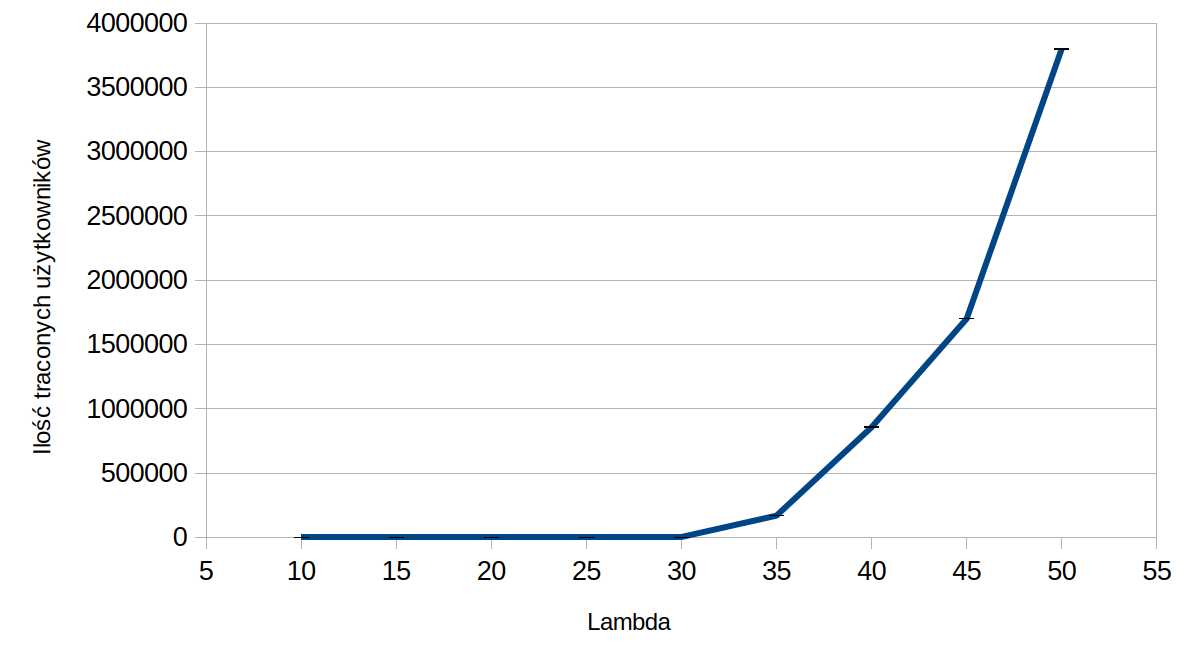
\includegraphics[scale=0.45]{img/dropped_users_by_lambda.png} 
\caption{Wykres liczby traconych użytkowników w funkcji wartości parametru $\lambda$}
\label{dropped_users_lambda}
\end{figure}

\newpage
\subsection{Wyznaczenie granicznej wartości progu L, dla której straty użytkowników są poniżej 5\%}\label{drop_rate_5_section}
Aby wyznaczyć wartość graniczną, uruchomiono symulację dla wartości progu L z zakresu $<5; 40>\%$, z krokiem 5. Każda próbka została uśredniona z 10 iteracji. W trakcie symulacji parametr $\lambda$ wynosił 35. Wynik symulacji przedstawiono na rysunku \ref{dropped_users_iter_l}. Z wyników symulacji wynika, że ilość traconych użytkowników w systemie nie zależy od wartości progu L. Eksperyment powtórzono dla wartości $\lambda = $ 40 oraz 50, których wyniki przedstawiono na rysunkach \ref{dropped_users_iter_l2} i \ref{dropped_users_iter_l3}.
W każdym przypadku różnice pomiędzy uzyskanymi wynikami są pomijalnie małe. Wynika to najprawdopodobniej z zastosowanego algorytmu usypiania i wybudzania stacji bazowych, który został zaprojektowany tak aby maksymalnie zminimalizować ilość traconych użytkowników w systemie. Analizując wykres zużycia zasobów stacji w czasie, przedstawionego na rysunku \ref{usage_over_time}, można zauważyć, że badana wartość utrzymuje się na w przybliżeniu stałym poziomie zależnym od współczynnika $\lambda$ w danej fazie. Aby wygenerować straty użytkowników przekraczające 5\%, parametr $\lambda$ powinien być duży, na przykład z zakresu $<50;70>$ użytkowników na sekundę, aby zapełnić bloki zasobów we wszystkich stacjach.
Zakres ten został wyznaczony osobnymi symulacjami, z wyłączoną logiką odpowiadająca za usypianie i wybudzanie stacji. Duża wartość parametru $\lambda$ jest także wymagana aby w systemie pojawiła się wystarczająca liczba użytkowników, aby przepełnić aktywne stacje, zanim zostanie wybudzona stacja uśpiona. Natomiast aby próg L, wskazujący poniżej jakiej wartości stacja bazowa może przejść w stan uśpienia, miał wpływ na przebieg symulacji, wartość parametru $\lambda$ musi być niska, aby zużycie bloków zasobów stacji spadło poniżej progu L. Jest to sprzeczne z postawionymi wcześniej założeniami i dlatego taka sytuacja nie zachodzi w systemie, dla podanych w treści zadania parametrów. Dlatego do dalszej części tego zadania, opisanego w sekcji \ref{get_params_section} przyjęto następujące parametry symulacji:
\begin{itemize}
\item Lambda = 43 użytkowników na sekundę
\item L = 20\%
\end{itemize}

\begin{figure}[h!]
\center
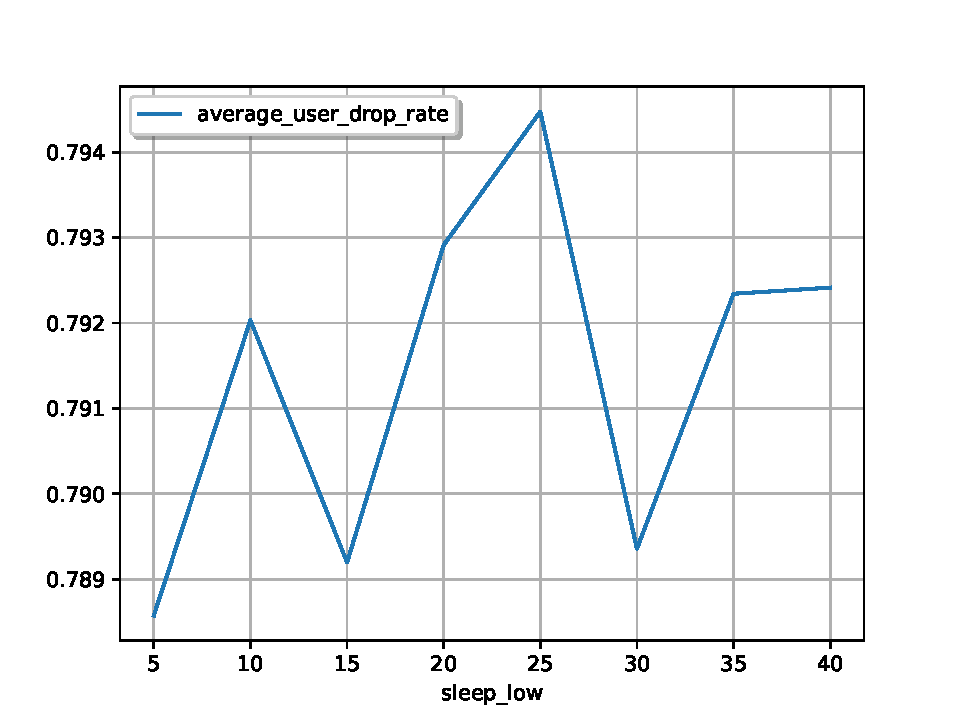
\includegraphics[scale=0.65]{img/drop_rate_lambda_35.pdf} 
\caption{Wykres procentu traconych użytkowników w funkcji wartości parametru L. W trakcie symulacji parametr $\lambda$ wynosił 35.}
\label{dropped_users_iter_l}
\end{figure}

\begin{figure}[h!]
\center
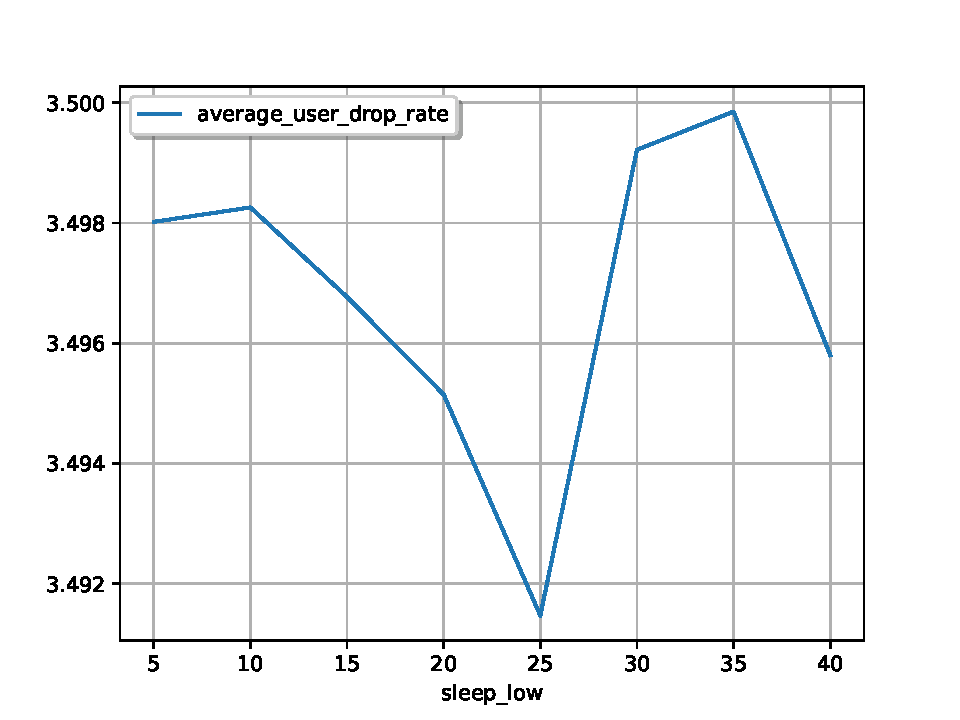
\includegraphics[scale=0.65]{img/drop_rate_lambda_40.pdf} 
\caption{Wykres procentu traconych użytkowników w funkcji wartości parametru L. W trakcie symulacji parametr $\lambda$ wynosił 40.}
\label{dropped_users_iter_l2}
\end{figure}

\begin{figure}[h!]
\center
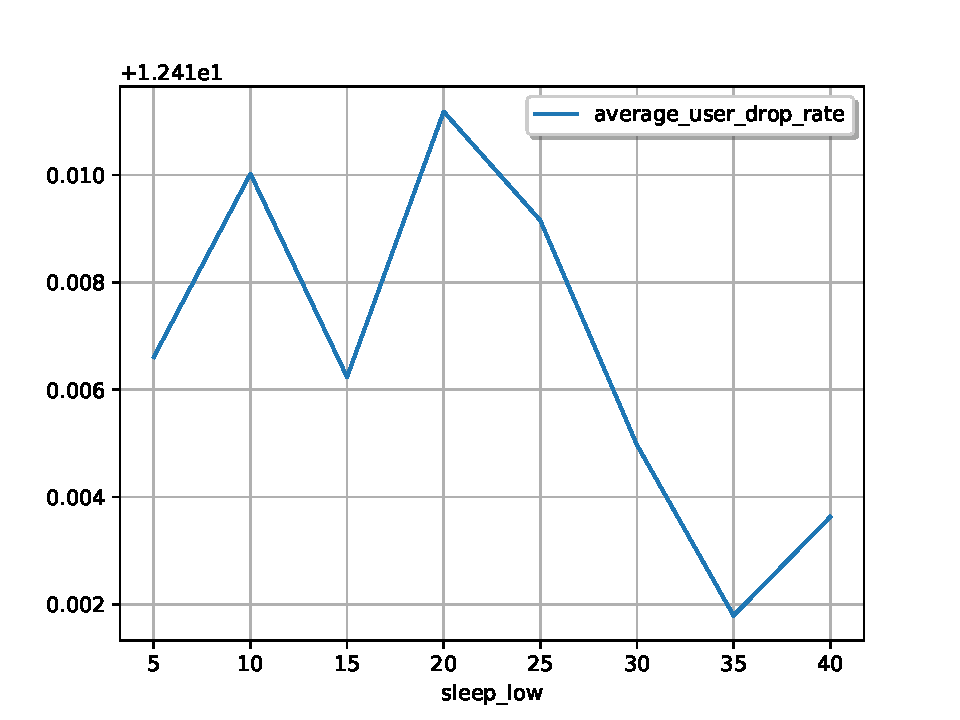
\includegraphics[scale=0.65]{img/drop_rate_lambda_50.pdf} 
\caption{Wykres procentu traconych użytkowników w funkcji wartości parametru L. W trakcie symulacji parametr $\lambda$ wynosił 50.}
\label{dropped_users_iter_l3}
\end{figure}

\begin{figure}[h!]
\center
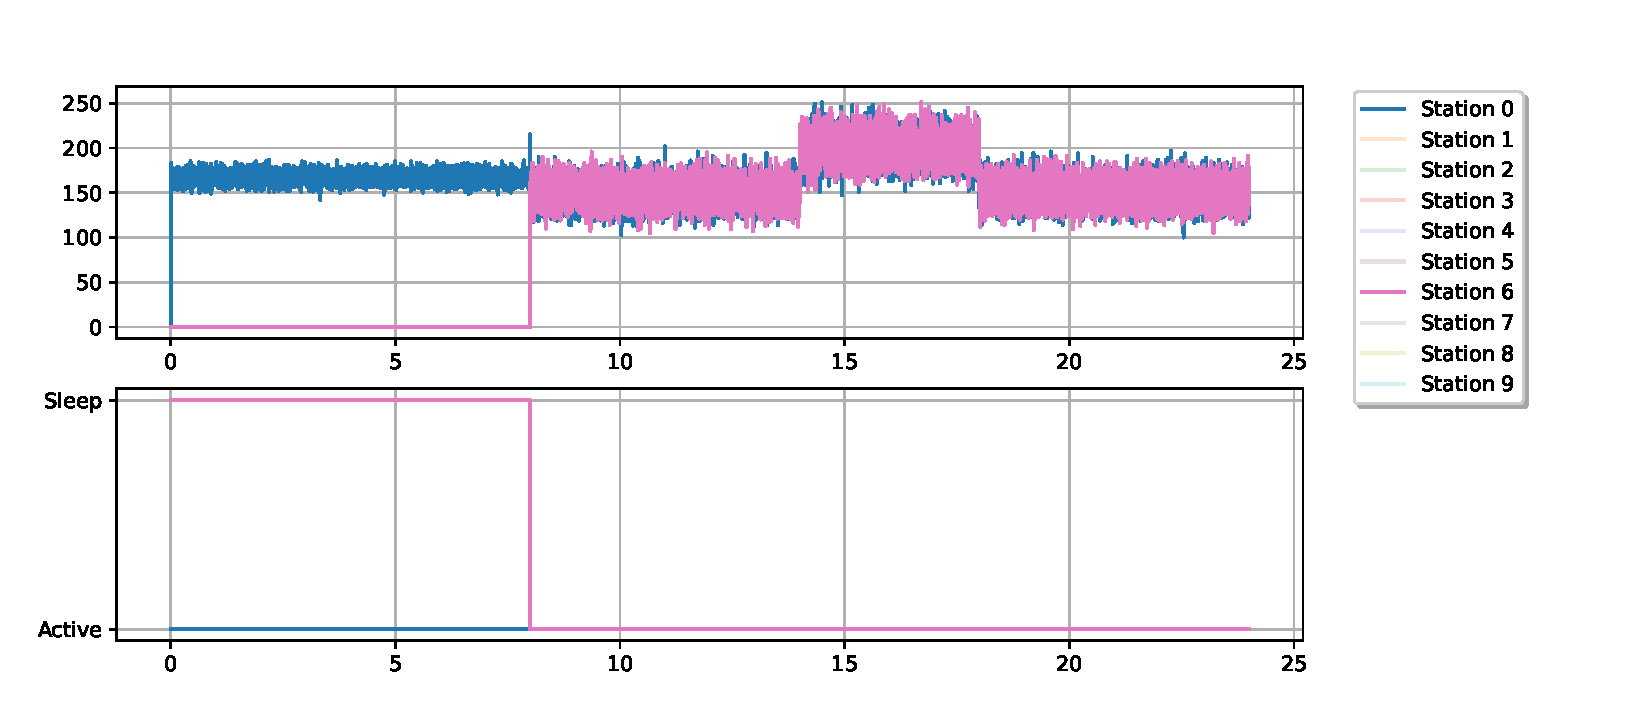
\includegraphics[scale=0.65]{img/usage_over_time.pdf} 
\caption{Wykres zużycia zasobów stacji bazowych nr 0 i 6 w funkcji czasu symulacji}
\label{usage_over_time}
\end{figure}

\newpage\newpage
\subsection{Wyznaczenie uśrednionych parametrów systemu} \label{get_params_section}
Uśrednione parametry systemu wyznaczono symulacją uśrednioną z 20 iteracji, gdzie parametr $\lambda$ wynosił 43 a próg L był równy 20\%. Wyniki symulacji oraz raport końcowy z programu przedstawiono odpowiednio w tabeli \ref{params_table} oraz na rysunku \ref{sim_results_average}. Ponieważ ilość użytkowników napływających do systemu była większa od pojemności stacji bazowych, wszystkie uśpione stacje zostały wybudzone w początkowej fazie symulacji, stąd średnia moc pobierana przez stacje wynosi 200W a średni czas uśpienia to 0\%. Parametry statystyczne zostały wyznaczone na podstawie wyników pośrednich, uzyskanych z użyciem przełącznika \emph{-{}-show-partial-results}, za pomocą wbudowanych funkcji programu \emph{Excel}.
\newline\newline
\begin{table}[]
\renewcommand{\arraystretch}{1.5}
\centering
\caption{Wyniki mierzonych parametrów systemu w każdej iteracji}
\label{params_table}
\begin{tabular}{|p{0.2\textwidth}|p{0.15\textwidth}|p{0.15\textwidth}|p{0.15\textwidth}|p{0.15\textwidth}|}
\hline
Iteracja & Średnie zużycie zasobów [\%] & Średni pobór mocy [W] & Średni procent traconych użytkowników & Średni czas uśpienia \\ \hline
0 & 84,891 & 200 & 4,899 & 0 \\ \hline
1 & 84,877 & 200 & 4,897 & 0 \\ \hline
2 & 84,899 & 200 & 4,902 & 0 \\ \hline
3 & 84,897 & 200 & 4,894 & 0 \\ \hline
4 & 84,863 & 200 & 4,890 & 0 \\ \hline
5 & 84,897 & 200 & 4,896 & 0 \\ \hline
6 & 84,863 & 200 & 4,905 & 0 \\ \hline
7 & 84,864 & 200 & 4,876 & 0 \\ \hline
8 & 84,890 & 200 & 4,909 & 0 \\ \hline
9 & 84,884 & 200 & 4,891 & 0 \\ \hline
10 & 84,898 & 200 & 4,890 & 0 \\ \hline
11 & 84,890 & 200 & 4,868 & 0 \\ \hline
12 & 84,873 & 200 & 4,896 & 0 \\ \hline
13 & 84,892 & 200 & 4,892 & 0 \\ \hline
14 & 84,896 & 200 & 4,880 & 0 \\ \hline
15 & 84,874 & 200 & 4,896 & 0 \\ \hline
16 & 84,893 & 200 & 4,895 & 0 \\ \hline
17 & 84,880 & 200 & 4,906 & 0 \\ \hline
18 & 84,901 & 200 & 4,896 & 0 \\ \hline
19 & 84,891 & 200 & 4,891 & 0 \\ \hline
Wartość średnia & 84,886 & 200 & 4,893 & 0 \\ \hline
Odchylenie standardowe & 0,0126 & 0 & 0,010 & 0 \\ \hline
Przedział ufności & 0,006 & - & 0,004 & - \\ \hline
\end{tabular}
\end{table}

\begin{figure}[h!]
\center
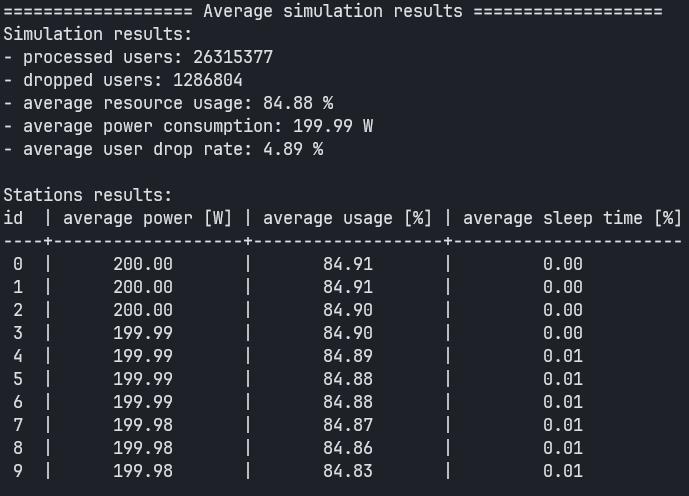
\includegraphics[scale=0.6]{img/sim_results_sleep_lambda_43.png} 
\caption{Raport wynikowy symulacji dla parametrów $\lambda$ = 43 oraz L = 20, uśredniony z 20 iteracji}
\label{sim_results_average}
\end{figure}

\newpage
\subsection{Wyznaczenie średniego zużycia energii w funkcji progu L} \label{power_l_plot}
Symulację wykonano dla wartości progu L z zakresu $<5:40>$ z krokiem równym 5, dla wartości parametru $\lambda$ = 20. Wyniki symulacji przedstawiono w tabeli \ref{power_usage_by_l} oraz na rysunku \ref{power_usage_lambda_sleep}. Każda próbka wykresu została uśredniona z 10 iteracji. Z analizy uzyskanego wykresu wynika że wraz ze wzrostem progu uśpienia L, dla niskich wartości $\lambda$, średni pobór mocy przez stacje bazowe maleje. Na rysunku \ref{usage_over_time_sleep} przedstawiono wykres zużycia zasobów stacji 0 i 7 w funkcji czasu. Stacja numer 7 została aktywowany po rozpoczęciu fazy największego ruchu (gdy współczynnik $\lambda\_coef$ = 1) oraz została wyłączona gdy generowany ruch zmalał. Dzięki temu średni pobór mocy w systemie zmalał, względem symulacji gdy próg uśpienia miał niższą wartość lub gdy logika odpowiedzialna za usypianie stacji była wyłączona.

\begin{table}[h]
\renewcommand{\arraystretch}{1.5}
\centering
\caption{Wyniki pomiaru średniego zużycia mocy w funkcji wartości parametru L}
\label{power_usage_by_l}
\begin{tabular}{|l|l|l|}
\hline
Próg L {[}\%{]} & Średnie zużycie mocy {[}W{]} & Przedział ufności \\ \hline
5 & 154,633 & 2,060 \\ \hline
10 & 153,566 & 1,833 \\ \hline
15 & 155,074 & 2,759 \\ \hline
20 & 155,949 & 3,213 \\ \hline
25 & 153,625 & 2,151 \\ \hline
30 & 149,099 & 1,698 \\ \hline
35 & 146,011 & 2,196 \\ \hline
40 & 139,263 & 0,989 \\ \hline
\end{tabular}
\end{table}

\begin{figure}[h!]
\center
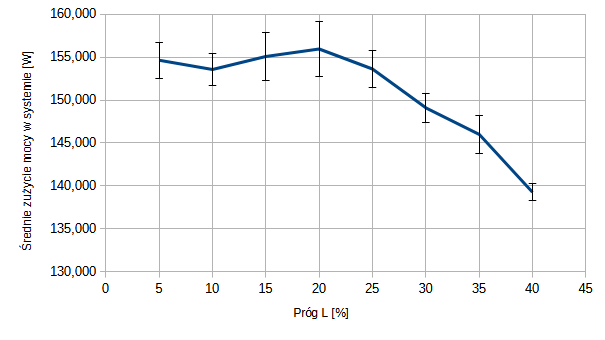
\includegraphics[scale=0.75]{img/power_by_l.png} 
\caption{Wykres średniego poboru mocy przez stacje bazowe w funkcji wartości progu L. W trakcie symulacji parametr $\lambda$ był równy 20}
\label{power_usage_lambda_sleep}
\end{figure}

\begin{figure}[h]
\center
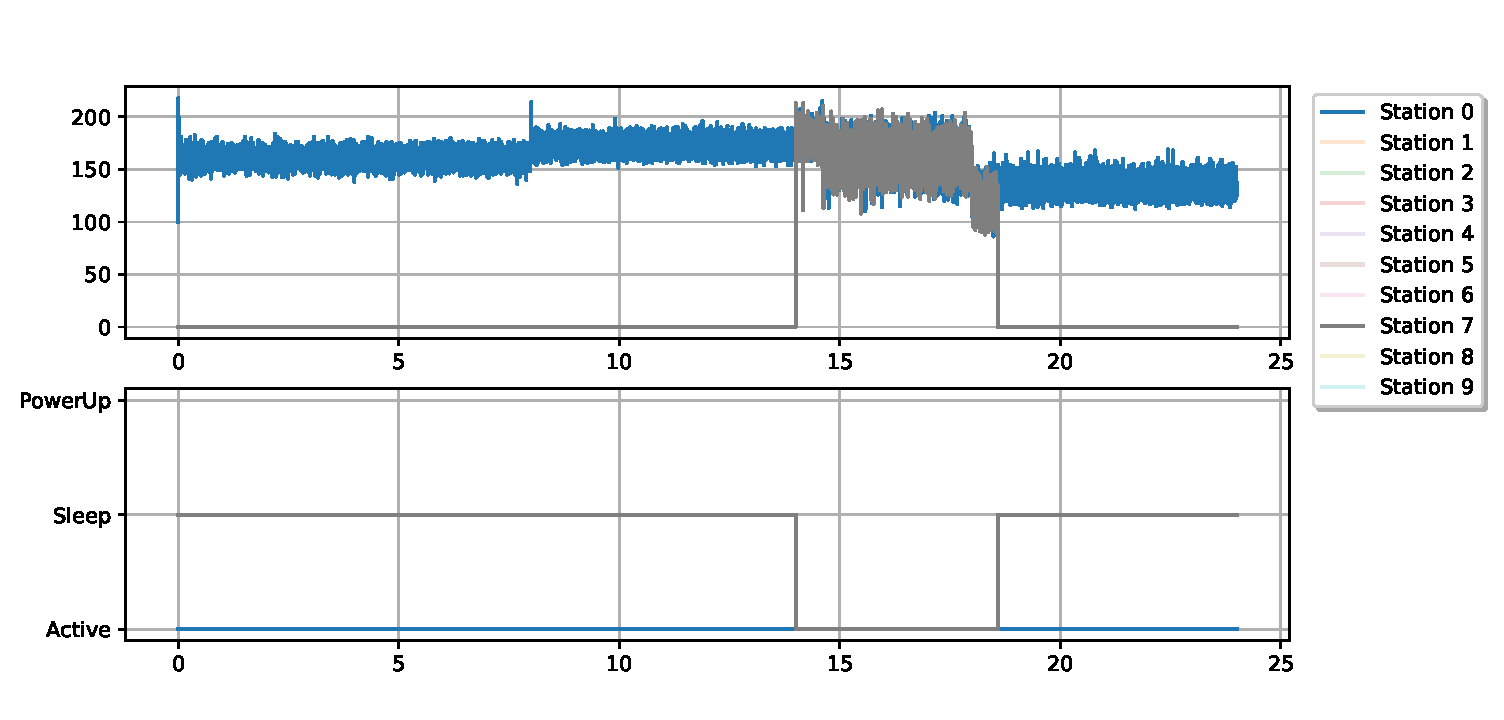
\includegraphics[scale=0.65]{img/usage_over_time_sleep.pdf} 
\caption{Wykres średniego poboru mocy przez stacje bazowe w funkcji wartości progu L}
\label{usage_over_time_sleep}
\end{figure}

\subsection{Wyznaczenie średniej ilości traconych użytkowników w funkcji progu L} \label{drop_l_plot}
Z przyczyn wymienionych w sekcji \ref{drop_rate_5_section}, liczba traconych użytkowników nie zależy od wartości progu L oraz, ponieważ w trakcie symulacji parametr $\lambda$ był równy 20, jest równa zero.

\begin{figure}[h!]
\center
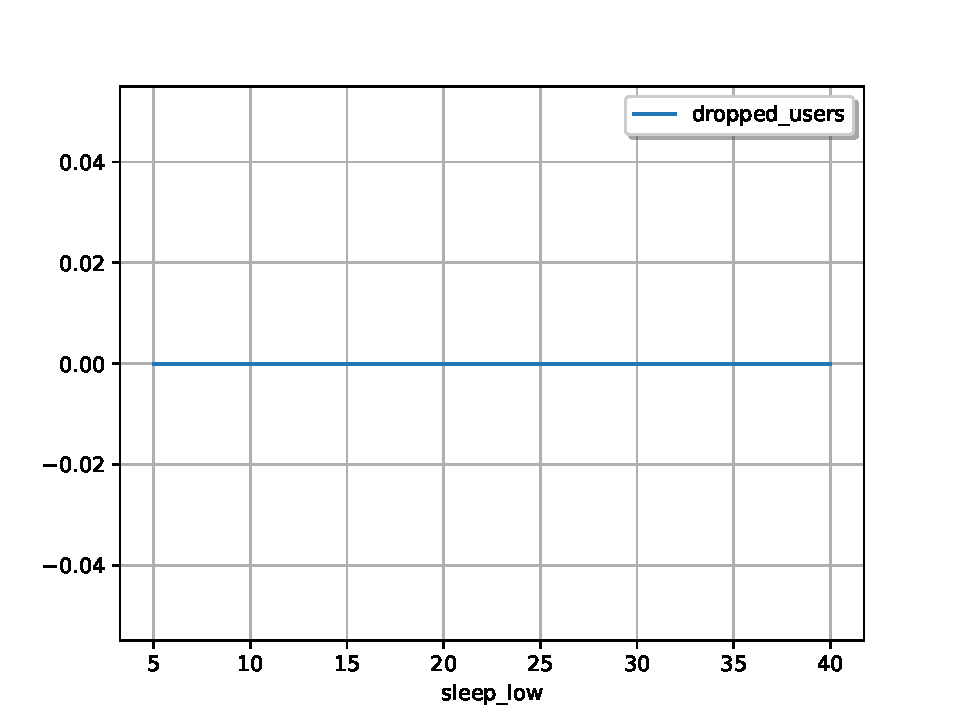
\includegraphics[scale=0.65]{img/dropped_users_lambda_20.pdf} 
\caption{Wykres średniego ilości traconych użytkowników w funkcji wartości progu L}
\label{drop_over_time_sleep}
\end{figure}
